\newpage
\section{Meshes and Clipping}
We want to represent objects of different nature ( curved, glossy ,bumpy...).A suitable encoding must be found to represent objects in a virtual environment.Using just a set of points is not enough to represent a solid object. Even using many vertices (~10000) can make the object look empty and more points would be computationally expensive.\\
Every solid object is stored by its boundary: what is \textbf{inside} vs what is \textbf{outside}.\\
Object geometries are encoded following mathematical models that represent \textbf{surfaces} through a set of parameters. Many models have been defined in literature : 
\begin{itemize}
\item \textbf{Meshes} (polygonal surfaces)
\item \textbf{Hermite surfaces}
\item \textbf{NURBS} (non uniform ration b-splines)
\item \textbf{HSS} ( hierarchical subdivision surfaces)
\textbf{Metaballs}
\end{itemize} 
All models are converted into \textbf{meshes} : its the only type of encoding that a low level rendering engine is capable of doing.\\
\subsection{Meshes}
A \textbf{mesh} is a polygonal surface that can be described by a set of contiguous polygons (cube, pyramid , prism are meshes ; cones,cylinders,spheres are not meshes but can be rendered as one using tricks shown later).\\
A polygon that describes a planar surface  portion of a surface is called a \textbf{surface}.\\
Sides of the polygons are called \textbf{edges} and correspond commonly to \textbf{intersection} of surfaces.\newpage
If every edge is \textbf{adjacent} to exactly \textbf{two} faces then the surfaces has a special topology called \textbf{2-manifold}.
Non 2-manifold surfaces usually represent non-physical objects and require special care (see below examples : solid with holes and lamina-faces)
\begin{figure}[H]
  \centering
  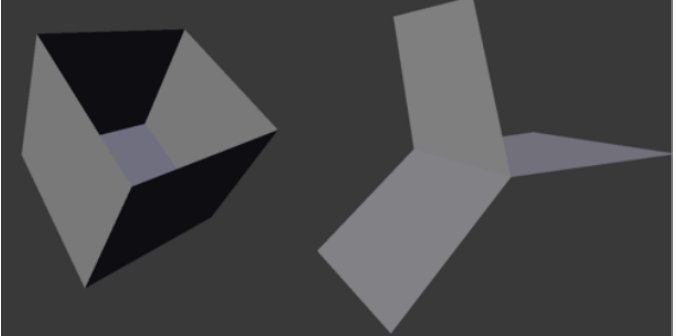
\includegraphics[width=.5\linewidth]{non2manifold}
\end{figure}
Sometimes non-2- manifold objects can be used to model very thin objects (pages...) or to obtain a special effect (opne box, magazine...). In these kind of situations the later presented \textbf{back-face culling} algorithm will \textbf{NOT} work.\\
Each polygon	 can be reduced to a set of \textbf{triangles} that shares some edges. A set of \textbf{adjacent triangles} is called a \textbf{mesh}.\\
Triangles are used because three points define a \textbf{planar surface} : otherwise if we had more points we could end up with different planes ( and thus different interpretations).\\
A polygonal surface (planar or not) is first \textbf{converted} into triangles known as \textbf{tessellation}. Polygon tessellation is not unique : several might be defined and not all are equivalent (some are better some are not).\\
A mesh representation of an object stores its surfaces with the set of polygons that delimit its boundary. Then the boundary polygons are in turn encoded as a set of contiguous triangles that share some edges.
\begin{figure}[H]
  \centering
  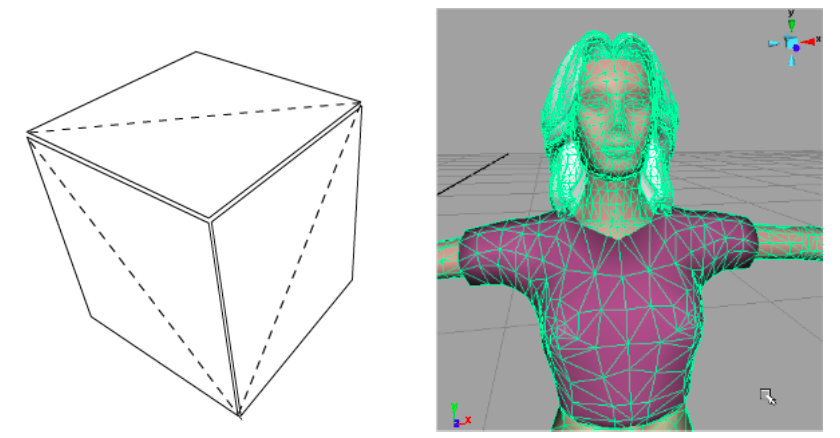
\includegraphics[width=.5\linewidth]{meshestex}
\end{figure}

\subsubsection{Mesh encoding}
Meshes are usually encoded as a \textbf{set of vertices}. The rendering engine uses such vertices to determine the end points of the triangles that compose the mesh

\begin{figure}[H]
  \centering
  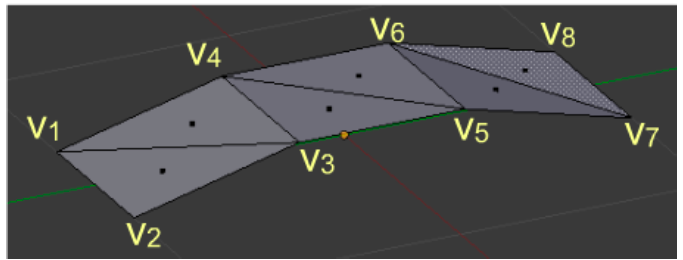
\includegraphics[width=.5\linewidth]{meshencoding}
\end{figure}
In the figure we have 3 surfaces divided into 6 triangles with and 8 vertices.
Each triangle has 3 vertices but instead of having 6x3 = 18 vertices we use 8 because 10 are shared
\begin{figure}[H]
  \centering
  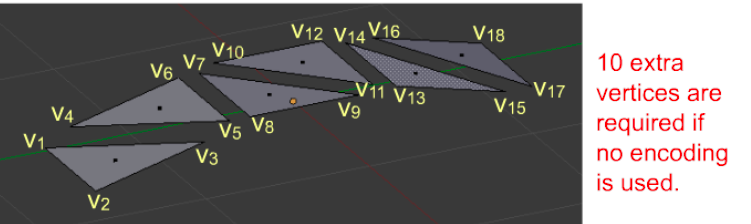
\includegraphics[width=.5\linewidth]{meshencodingv}
\end{figure}

Three main types of mesh-encoding are:
\begin{itemize}
\item \textbf{Triangle Lists}
\item\textbf{ Triangle Strips}
\item \textbf{Triangles Fans}
\end{itemize}

\begin{description}
\item[Triangle lists]\hfill\\ 
Triangle lists do \textbf{not} exploit any \textbf{sharing vertices} and encode each triangle \textbf{separately}. They are used to encode \textbf{unconnected} triangles
\begin{figure}[H]
  \centering
  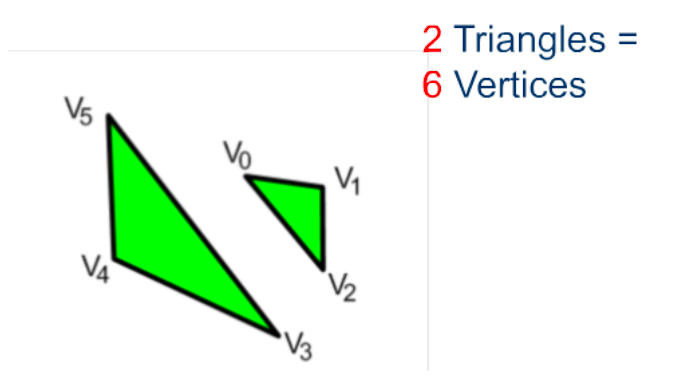
\includegraphics[width=.5\linewidth]{trianglelists}
\end{figure}

\item[Triangle strips]\hfill\\
Triangle strips encode a \textbf{set of adjacent} triangles that define a band-like surface.The encoding begins by considering the first two vertices. Then each new vertex is connected to the previous two.
\begin{figure}[H]
  \centering
  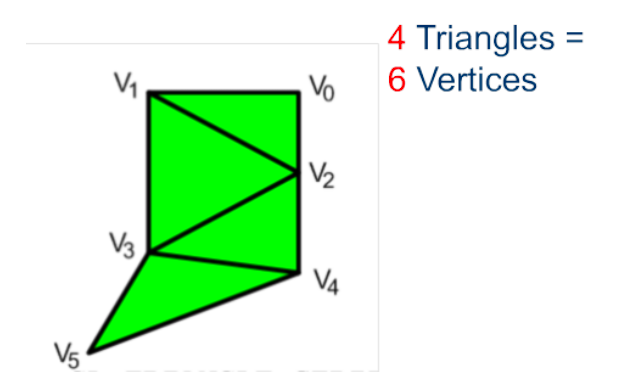
\includegraphics[width=.5\linewidth]{trianglestrips}
\end{figure}

\item[Triangle fans]\hfill\\
Triangle fans encode polygons where all the triangles share a \textbf{vertex}.The first two vertexes are specified independently.Then each new vertex connects both the previous one and the first of the list.
\begin{figure}[H]
  \centering
  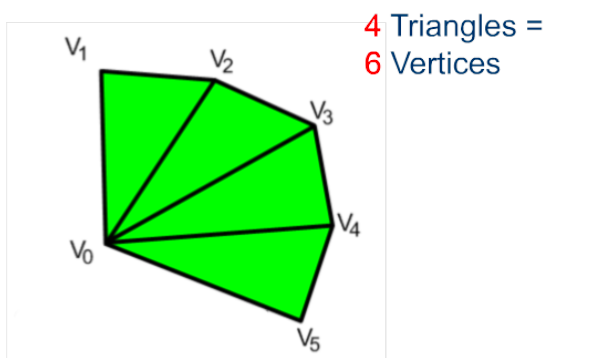
\includegraphics[width=.5\linewidth]{trianglefans}
\end{figure}
\end{description}

\subsubsection{Indexed Primitives}

Triangle lists and strips can \textbf{save} some memory most of the times. Sometimes though they are not an advantage even if the topology would seem to be appropriate. This is due to the fact that often vertexes are \textbf{repeated} .Another reason is that vertexes are encoded by more parameters than just their coordinates (i.e. normal vector and texture mapping) : you can save memory only if shared vertexes are \textbf{identical} with respect to all parameters , otherwise different encodings for that vertex are required.\\
Many primitives cannot be encoded with a single triangle strip/fan so many vertexes can still be shared between different strips/fans. \textbf{Indexed primitives} allow reducing the cost of replicating the same vertex between different lists/strips/fans. 
\begin{figure}[H]
  \centering
  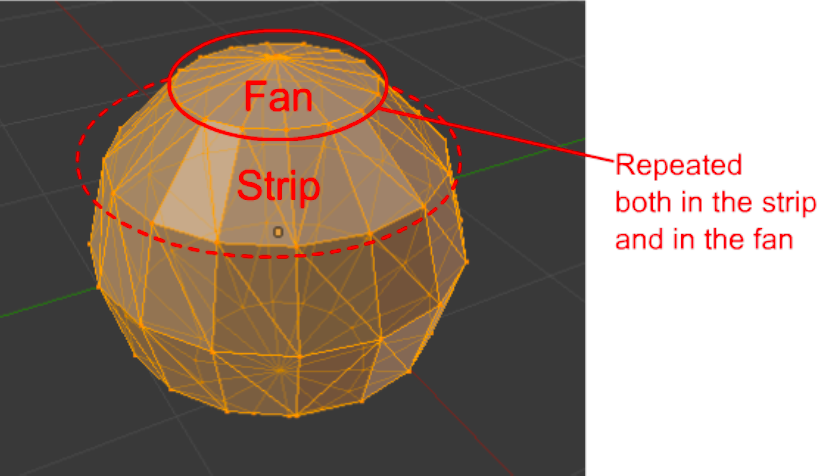
\includegraphics[width=.5\linewidth]{spherefanstrip}
\end{figure}
In this case the cap of the sphere is encoded using a fan, and the rings using strips. The points connecting fan and strip are shared , so they are encoded two times. This is also true for the first ring and second ring , the second ring and the third ring and finally the third ring and the lower cap.A solution to this are \textbf{Indexed primitives}.They are defined by two arrays:
\begin{itemize}
\item \textbf{Vertex Array}:\\
Contains the definitions/positions of the different vertexes.For example a cube will have a list of 8 (x,y,z) elements.
\item \textbf{Index Array}:\\
Are used to \textbf{indirectly} specify the triangles. For example a cube has 6 faces so we have 12 triangles. So in the index array we have 12 elements (a,b,c) where a,b,c are the indexes of the vertex array composing that triangle. 
\end{itemize}

\begin{description}
\item[Example]\hfill\\
Consider a cube encoded in strip lists. We have 6 faces, 12 triangles each has 3 vertexes using three coordinates each is a float (4B) so :
$$ 6*2*3*3*4 = 432 Bytes$$
If the cube is encoded in triangle strips only 14 vertexes are required
\begin{figure}[H]
  \centering
  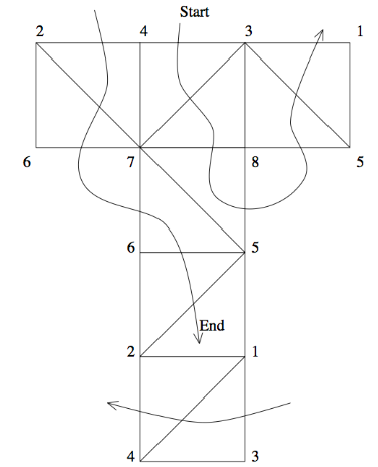
\includegraphics[width=.4\linewidth]{cubestrips}
\end{figure}
$$ 14*3*4=168$$
Using indexed primitives we need 8 vertexes (the ones of the cube) and 36 indices ($\approx$ 1B):
$$ 8_{vert}*3_{xyz}*4_{float} + 6_{faces}*2_{tri}*3_{vert}*1_{byte}= 132 Bytes$$
By using indexed primitives with triangle strips we can reduce the size even more:
$$ 96+14=110 Bytes$$
\end{description}

\subsection{Clipping}
The triangles of a mesh can intersect the boundary of the screen and can be partially shown. The clipping process is performed \textbf{after} the projection transform but \textbf{before} the normalization step (in other word it is performed on the \textbf{clipping } coordinates)\\
In 3D space clipping is performed against the viewing frustum :
\begin{figure}[H]
  \centering
  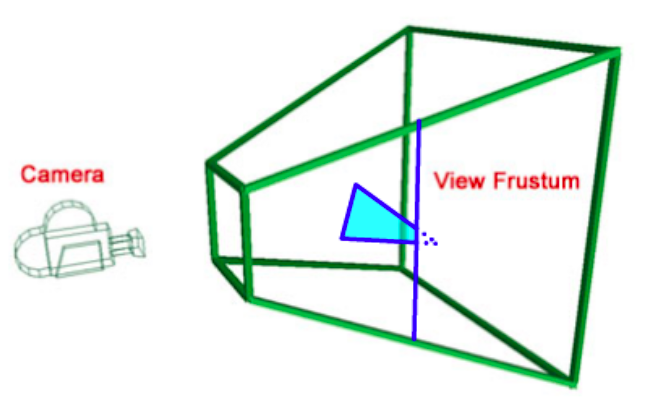
\includegraphics[width=.5\linewidth]{clippingfrustum}
\end{figure} 
The equation of a plane is $$ n_x x + n_y y +n_z z + d = 0$$ where $n_x,n_y,n_z$ represent the \textbf{normal} to the plane. The constant term d  defines the distance from the origin (0 if the plane passes through the center of axis). The equation divides the 3D space into two regions called \textbf{half space}:
$$ n_x x + n_y y +n_z z + d > 0$$ $$ n_x x + n_y y +n_z z + d < 0$$
The frustum is convex solid an can be determined by 6 half spaces. For each of these 6 half-spaces the above equations are used to determine if a points belong the correct half space.This can be simplified by a scalar product of two vector:
\begin{itemize}
\item  $n=(n_x,n_y,n_z,d)$ identifies the plane
\item  $p=(x,y,z,1)$ for the point
\end{itemize}
$$ n_x x + n_y y +n_z z + d =  \to n \cdot p = 0$$
The six normal vectors can be computed together with the projection matrix.However if clipping is performed into clipping space, since coordinates are meant to be inside the frustum if between -1 and 1, the six vector become very simple:
\begin{figure}[H]
  \centering
  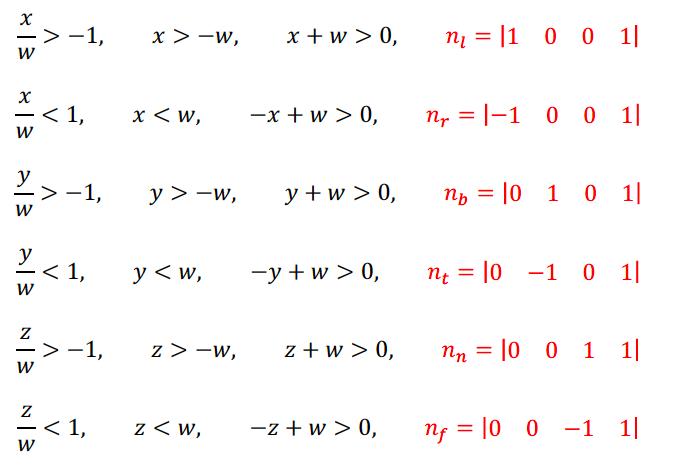
\includegraphics[width=.5\linewidth]{clippingvec}
\end{figure}
So points will be inside the frustum if :
\[
\boxed{p \cdot n_v > 0 \quad \forall v \in \{l,r,t,b,n,f\}}
\]

\subsubsection{Clipping triangles}
Clipping points is easily done given the normal vectors and the points in space with the above formula. In triangles the same principle is applied for all its vertex. But how is a triangles rendered inside the frustum when clipping is performed on one or more vertexes?
\begin{figure}[H]
  \centering
  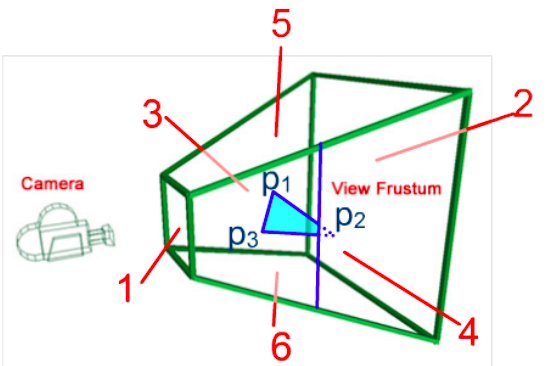
\includegraphics[width=.5\linewidth]{clippingtri}
\end{figure}
As shown the triangle and the frustum face are intersected . Computationally this is done by the \textbf{Sutherland-Hodgman Algorithm}.\\
Focusing one on the figure above we have a face defined by its vector $n_v$ and the three vertexes of the triangle $p1,p2,p3$ : 
$$ d_1 = p_1n_v $$
$$ d_2 = p_2n_v $$
$$ d_3 = p_3n_v $$
Trivial cases all points are inside/outside ($d_i >0$ / $d_i<0$). If all points are outside the algorithms stops.If the they are all positive the algorithms moves to the next face.\\
On the other hand if two points are on the outside ($p_2,p_3$) and one the inside ($p_1$) the two \textbf{intersections} $p'_2,p'_3$ are computed using \textbf{interpolation}. 
\begin{figure}[H]
  \centering
  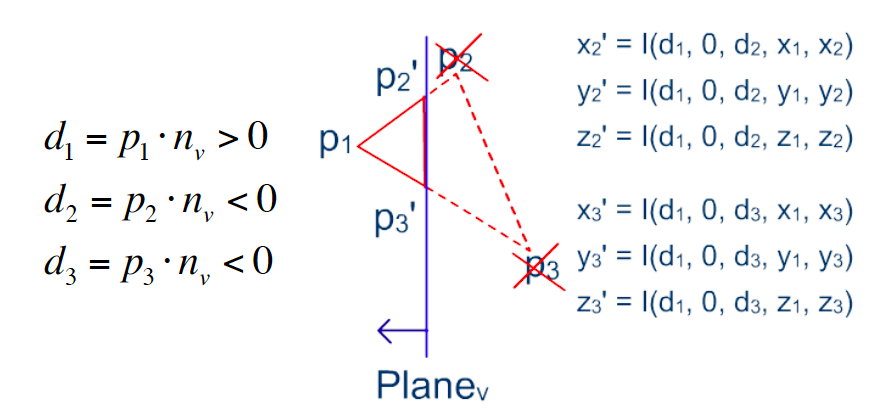
\includegraphics[width=.5\linewidth]{clippingex1}
\end{figure}
The distance from plane $d_2,d_3$ are used as interpolation factors: 
$$ p'_2= (x'_2,y'_2,z'_2)$$
$$ x'_2 = I(d_1,0,d_2,x_1,x_2)$$
$$ y'_2 = I(d_1,0,d_2,y_1,y_2)$$
$$ z'_2 = I(d_1,0,d_2,z_1,z_2)$$

$$ p'_3= (x'_3,y'_3,z'_3)$$
$$ x'_3 = I(d_1,0,d_3,x_1,x_3)$$
$$ y'_3 = I(d_1,0,d_3,y_1,y_3)$$
$$ z'_3 = I(d_1,0,d_3,z_1,z_3)$$
In clipping space also the fourth coordinate w must be interpolated!
f two points are on the inside ($p_2,p_3$) and one the outside ($p_1$) we have a more complex situation : two triangles are formed.
\begin{figure}[H]
  \centering
  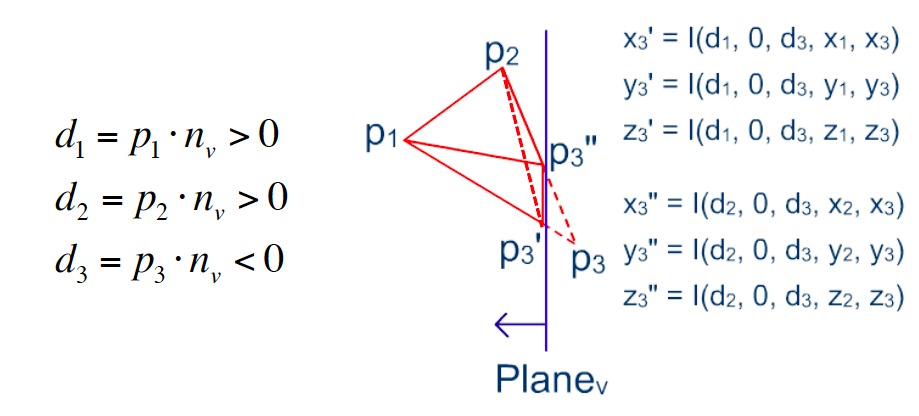
\includegraphics[width=.5\linewidth]{clippingex2}
\end{figure}
The algorithm terminates when all faces have been checked for clipping or all three points are outside the frustum.\\
The algorithms is simple but can produce many triangles since it can potentially double at every check